\documentclass[10pt,norsk,a4paper]{article}
\usepackage[utf8]{inputenc}
\usepackage[T1]{fontenc}
\usepackage[norsk]{babel}
% PDF-relatert
\usepackage{hyperref,pdfpages,hypcap}
\hypersetup{colorlinks=true,allcolors=.}
\newcommand\fhref[2]{%
	\href{#1}{#2}\footnote{\url{#1}}%
}
% Andre pakker
\usepackage[cm]{fullpage}
\usepackage{parskip,multicol,textcomp,amssymb,graphicx,color,enumitem}
% - Korreksjon av fotnoter i seksjoner/overskrifter
\usepackage[stable]{footmisc}
% - Skrifttype
\usepackage[bitstream-charter]{mathdesign}


\title{Generalforsamling \\
	Våren 2018\\[3cm]
	
\includegraphics[width=0.5\textwidth]{cyb-logo.eps}\\[-.5cm]}
\date{2.\ mai 2018}
\author{Cybernetisk Selskab}

% Blank header, samt footer med side x av y
\usepackage{fancyhdr}
\pagestyle{fancy}
\renewcommand{\headrulewidth}{0pt}
\fancyhead{}
\cfoot{Side~\thepage\ av~\pageref*{lastpage}}


\begin{document}

\maketitle{}
\newpage
\tableofcontents


\section{Valg av møteleder}

\section{Valg av referent}

\section{Valg av protokollunderskrivere}

\section{Valg av tellekorps}

\section{Godkjenning av innkalling}

\section{Godkjenning av dagsorden}

\section{Semesterberetninger}
\subsection{Semesterberetning ved leder}
\textit{Kjære interne, medlemmer og studenter,}
\begin{multicols}{2}
Nok et semester har kommet og gått, og vi kan nok en gang si oss fornøyd med forrige semester. Som alltid
har vi hatt noen utfordringer: vi har slitt litt med nytt kassasystem, og vi har rekruttert færre interne enn hva vi hadde ønsket oss. Selv med dette har vi fått til mye nytt og mye vi kan skryte av.

Dette vårsemesteret har vi slått en ny medlemsrekord for et vårsemestre. Vi har i skrivende stund 663
medlemmer, noe som er 37 flere enn på samme tid i fjor. Dette kan henge sammen med at vi har hatt et veldig høyt aktivitetsnivå, med arrangementer nesten hver eneste dag. Om vi ser på april, så er det aktiviteter på 26 av 30 dager i Escape eller i regi av CYB andre steder.

En av de store begivenhetene CYB har vært med på dette semesteret er stiftelsen av \textit{Forente IT-foreninger}. Dette er et samarbeidsforum for IT-studentforeninger i Norge. Vi møttes for første gang her i Escape 21.\ april, hvor vi diskutere temaer som studieoppbygging, frafall av studenter, studentpolitikk og kontakt med arbeidslivet. Vi håper dette kan være en tradisjon som blir opprettholdt, og sammen med de andre deltagerne ble det bestemt at vi skal møtes på nytt allerede til høsten i Trondheim.

Vi har også startet i det små med arbeidet til CYB50. Her gjenstår det mye arbeid, og vi trenger ildsjeler til å få arrangert jubileet. Jeg oppfordrer alle interne til å melde interesse til hovedstyret.

Det siste vi har jobbet med, spesielt mot slutten av semesteret, er kommunikasjon mellom studentforeningene ved Ifi opp mot administrasjonen på instituttet. Etter at både sentrale personer i studentmiljøet og i administrasjonen har blitt byttet ut, så har mange av de personlige relasjonene blitt borte. Administrasjonen virker også litt underbemannet og dette har gjort det tidkrevende og vanskelig å få gjennomslag oppover i etasjene. Som instituttforening mener jeg at det er naturlig at CYB står i fronten for arbeidet med å forbedre samarbeidet med instituttet fremover. 

\end{multicols}

Jeg ønsker å takke for meg, og samarbeidet i hovedstyret, samtidig som jeg ser fram til å bidra videre som intern.

\textbf{Andreas Hansen},\\
leder \\
\date{25.\ april 2018}
\newpage


\subsection{Semesterberetning ved kjellermogul}

\begin{multicols}{2}
Semesteret startet med et positivt smell, hvor vi fikk både nytt kassesystem og en oppgradering av
tappeanlegget. Oppgraderingen av tappeanlegget førte til en del problemer i starten, men etter en del frem og tilbake med tekniker fra Aass så ble mer eller mindre alle problemene løst. Aass har nå fått seg en teknikker som jobber fast i Oslo, noe som har gitt oss en del bedre oppfølging og vedlikehold gjennom semesteret. Det nye kassasystemet viste seg derimot å bli et større problem. Her har vi brukt mye tid på å få svar fra Ajour, men ikke til noe særlig nytte. Slik det er nå fungerer ikke integrasjonen mot tripletex, og det er diverse andre problemer som ikke lar seg fikse uten videre. Grunnet dette ga KS Fredrik Magnussen et mandat til å jakte på et nytt og bedre system. Det viser seg at det ikke bare er vi som sliter, og har nå fått med oss RF, Kjelleren og Uglebo på saken. Forhåpentligvis finner vi et nytt og mer robust system.

Forholdsvis tidlig i semesteret ble vi kontaktet av Hansa Borg, som ønsket at vi skulle bytte til dem. Etter
et positivt møte med en salgsperson fra dem fikk vi omsider et knakende bra tilbud. Siden vi føler såpass
mye tilhørighet til Aass kontaktet Tor-Aksel vår kontakt, som ønsket et møte så kjapt som dagen derpå. Utfallet av dette møtet gikk over all forventning, og førte til en avtale som gir oss mange økonomiske fordeler med mer. Blant annet fikk vi endelig lov til å ha et “aktivitetstårn”, som teknikeren fra Aass monterte knappe uken etter at avtalen var signert.

Videre har undertegnede sendt inn en søknad til \textit{Sparebankstiftelsen DNB}, hvor vi har søkt om 80~000
til en ny espressomaskin. Som med mesteparten av utstyret i Escape begynner også denne å synge på siste
verset. Derfor kommer vi forhåpentligvis til å bytte denne ut i løpet av neste semester. Utover dette har
det vært små reperasjoner på alt fra oppvaskmaskin til kjøleskap. Den siste av kaffetrakterne ble også
byttet ut da den eldste av dem sviktet, og måtte umiddelbart på gamlehjem.

For å gjøre Escape litt mer koselig har det blitt kjøpt inn noe nytt inventar. Det ble blant annet kjøpt inn
to nye hyller; en stor til brettspillene, og en litt mindre som skal fylles med bøker fra
realfagsbiblioteket. De er vi for øvrig i samtale med om å få til et offisielt, og ikke minst nærmere,
samarbeid med. Det har også blitt kjøpt inn noen praktiske planter for å kryddre lokalet litt.

Torsdagsklubben er som forrige semester noe vi har fortsatt med. Det har vært litt varierende kvalitet på
arrangementene, og dermed har også deltagelsen vært varierende. Likevel har det har vært en positiv erfaring
å ha med seg, da flere funker får opplæring i noe litt utenom tapping av øl. I den sammenheng har det også
blitt utarbeidet en liten “standardmeny” for spritholdige drinker. Forhåpentligvis er Torsdagsklubben noe
som vil plante seg blant klientellet som et fast tilbud, hvor oppmøtet på sikt, forhåpentligvis, vil øke. Ellers har det vært svært høy aktivitet i Escape, hvor det har vært arrangert alt fra brettspill til et stort antall utlån.

En ting som har vært litt problematisk dette semesteret for driften av Escape, er internmassen. Vi har rett
og slett ikke vært flinke nok til å rekruttere dette semesteret, og det har ført til at få folk har jobbet
veldig mye. Selvsagt er det positivt at vi har såpass flinke og engasjerte interne, men det kunne gjerne ha
vært fler, tatt behovet i betraktning.

Alt i alt har dette semesteret gått rundt som vanlig, med en del små og store forandringer. Internt i KS
kunne kommunikasjonen vært litt bedre. Dette er forhåpentligvis noe de som sitter videre, og de nye som
kommer inn kan jobbe sammen om for å forbedre. Videre er det noen ting som burde bli gjort neste semester:
\begin{itemize}
		\item Rekruttere bedre i starten av semesteret (studiestartuka er en gullgruve)
		\item Finne en bedre kasse, om mulig
		\item Bedre oppfølging av rutiner
		\item Bedre intern kommunikasjon
\end{itemize}
\end{multicols}
Vi sees i Escape!

\textbf{Adrian Helle}, \\
kjellermogul \\
\date{24.\ april 2018}

%\newpage

\section{Kasserer orienterer}
\subsection{Regnskapets tilstand}
Kasserer presenterer regnskapet.


\subsection{Revidert budsjett for høsten 2018}
Kasserer presenterer budsjett.


\section{Kontigentfastsettelse}
Hovedstyret foreslår å holde medlemskontigenten på kr.~40,-.

\section{Forslag til endring av stemmemetodikk}

Et samlet hovedstyre ønsker å legge fram et forslag om å endre stemmemetoden ved valg på generalforsamlinger, samt umiddelbar ikrafttredelse, hvor sistnevnte er avhengig av at det primære vedtektsforslaget godkjennes. Hovedstyret støttet et forslag om \textit{Instant-runoff stemmegivning}, ettersom denne varianten er hva preferansevalg\footnote{Også kjent som STV:\ single transferable vote.} er tilnærmert likt når man kun skal velge én vinner. Ordlyden i vedtektsforslaget nedenfor er endret til å presisere preferansevalg i henhold til UiOs reglement, da dette allerede brukes for rektorvalget, studentparlamentet, og samtidig er sterkt og utfyllende i gjennomførelsen.

\begin{description}[style=nextline]
	\item[Hvorfor bytte vekk fra simpelt flertall?]
		Simpelt flertall er sårbar for taktisk stemmegivning, bortkastede stemmer, m.m., og gir et vesentlig mindre representativt valgresultat. Dette oppstår med en gang det er mer enn to kandidater til et gitt valg.

	\item[Hvordan vil valget utføres med preferansevalg?]
		Gjennomførelsen av valget er veldig godt dokumentert i valgreglementet for Universitet i Oslo, og kan brukes til vårt formål, selv om vi for eksempel velger inn én person for et gitt verv.
		

\end{description}

\textbf{Ytterligere detaljer kommer på oppdatert dagsorden, i lag med presentasjon på generalforsamlingen.}

\subsection{Forslag til endring av §8a til fordel for preferansevalg}

Erstatter \textit{simpelt flertall} med \textit{preferansevalg, jf.~Valgreglement for Universitet i Oslo §13}.

\begin{enumerate}
	\item[§8 a] Valgbare til alle styrer er alle medlemmer i henhold til §2 og informatikkstudenter ved Universitetet i Oslo. Alle valg avgjøres ved \textcolor{red}{preferansevalg, jf.~\fhref{https://www.uio.no/om/regelverk/orgadm/valgreglement.html\#vedlegg-2}{Valgreglement for Universitet i Oslo §13}}.
\end{enumerate}

\subsection{Forslag til umiddelbar ikrafttredelse}

Ovenfornevnte forslag foreslås umiddelbart ikrafttredelse på generalforsamlingen.
Konsekvensen av dette er at følgende valg hvor tre eller flere kandidater stiller vil merke en forskjell i valggjennomførelsen på grunn av \textit{preferansevalget}.



\section{Valg}

\begin{minipage}[t]{0.49\textwidth}
\subsection{Hovedstyret} %TODO Oppdater listen med verv
Man velges inn i hovedstyret for ett år av gangen.

\subsubsection{Leder}
\subsubsection{Nestleder}
\subsubsection{Arrangementssjef}
\subsubsection{Rekrutteringsanasvarlig}

\end{minipage}
\begin{minipage}[t]{0.49\textwidth}
\subsection{Kjellerstyret} %TODO Oppdater listen med verv
Alle verv som er til valg i kjellerstyret gjelder for ett semester av gangen.

\subsubsection{Innkjøpsansvarlig}
\subsubsection{Barsjef}
\subsubsection{Kafésjef}
\subsubsection{Teknisk ansvarlig}
\subsubsection{DJ-sjef}
\subsubsection{Utlånsansvarlig}
\subsubsection{Arrangementskoordinator}

\end{minipage}

\newpage

\section{Vedtektsendringer}
Følgende to, og eksklusive, forslag for vedtektsendringer ligger fremme.

\subsection{Første variant: Endring i forbindelse med krav om Ifi-foreninger}\label{sec:ifi-forslag}

For å begrense, samt formalisere, hvilke foreninger som er en ``Ifi-forening''
har Ifi satt sammen noen vedtekter som studentforeningene må følge.  Per dags
dato følger ikke Cybernetisk Selskab §1c\footnotemark. Det ble lagt frem et
forslag av hovedstyret på vårens og høstens generalforsamling i fjor, for å
endre våre vedtekter, slik at vi ikke bryter med kravet.


\footnotetext{Etter manglende vedtektsfesting av to-tredelers Ifi-studenter i hovedstyret.}

Dette ble da ikke vedtatt da forsamlingen først konkluderte med at de nye vedtektene var for åpne og uklare.
Forsamlingen ønsket at hovedstyret skulle komme med et nytt forslag til høstens generalforsamling, hvor et
nytt forslag ble presentert. Dette ble ei vedtatt, da man ønsket å formelt starte søknadsprossen i henhold
til §3c.

Etter at hovedstyret har vært i kontakt med Studielaben, både skriftlig og i et møte, fikk vi avslag på vår
søknad. Studielaben signaliserte klart at deres tanker om søknaden var gjort opp før møtet vårt, og
var ikke særskilt imøtekommende med tanke på eventuelt kompromiss gitt vår posisjon som en forening med
en studentkjeller.

For å forebygge videre utfall, samt sikte på bedre samarbeid, legger vi fram et forslag som fleksibelt, og
forholdsvis enkelt, oppnår og imøtekommer prinsippet og kravet. Vi forstår fortsatt tanken bak kravet, og
hvor det stammer fra, samtidig som den manglende samarbeidsviljen når vi er i en særskilt rolle er
noe uheldig, og ikke ønsker å signalisere et ønske om mindre mangfold i foreninger.

Begge endringsforslagene hører sammen og stemmes over i lag.

\subsubsection{Forslag til ny paragraf: §5h}
\begin{enumerate}
	\item[§5h] Minimum to-tredeler av hovedstyret skal bestå av studenter som enten (1) er tilknyttet et eller flere studieprogrammer ved \textit{Institutt for informatikk}, eller (2) som tar ett eller flere IN- eller INF-fag.
\end{enumerate}

\subsubsection{Forslag til endring av paragraf: §8a}
\begin{enumerate}
	\item[§8a]
		Valgbare til alle styrer er alle medlemmer jf.~§2 og informatikkstudenter ved
		Universitetet i Oslo. 
		\textcolor{red}{%
			Om valgresultatet er ugyldig jf.~§5h kan
			generalforsamlingen velge inn ytterligere styremedlemmer for å utjevne og imøtekomme
			styrebalansen, selv om dette strider mot øvre grense jf.~§5d.
		}Alle valg avgjøres ved \textit{simpelt flertall}.
\end{enumerate}


\subsection{Andre variant: Endring i forbindelse med krav om Ifi-foreninger}

Som i~\ref{sec:ifi-forslag} ligger det et alternativt forslag fremme for å løse problematikken med \textit{Vedtekter for Ifi-foreninger}, fremmet av Nikolas Papaioannou.

\begin{quote}
	\ldots\ Målet er å legge in en myk versjon av det Studielaben ved Institutt for informatikk prøver å få oss til å oppnå, samtidig som det også løser eventuelle problemstillinger rundt ugyldige generalforsamlinger.
\end{quote}

Begge endringsforslagene hører sammen og stemmes over i lag.

\subsubsection{Forslag til ny paragraf: §5h}

\begin{itemize}
	\item[§5h] Hovedstyret skal strebe mot å opprettholde en minimumsandel på to tredjedeler studenter som enten er tilknyttet et eller flere studieprogrammer ved Institutt for informatikk, eller som tar ett eller flere IN- eller INF-fag.
\end{itemize}

\subsubsection{Forslag til ny paragraf: §5l}
\begin{itemize}
	\item[§5l] Hvis §5h ikke er oppfylt etter en generalforsamling skal hovedstyret drøfte på neste
		ordinære styremøte om det er nødvendig med en eventuell etterfylling opp mot grensen
		jf.~§5d.
\end{itemize}

\section{Æresmedlemskap}

\section{Utdeling av pins}

Arkivar deler ut pins.

\section{CYB50}

CYB har 50.~årsjubileum februar 2019, og trenger i den sammenheng frivillige til dette formålet. Leder for komitèen orienterer litt rundt planer sålangt.

Interesse for deltagelse i arrangeringen kan sendes til \textbf{cyb50@cyb.no}.

\part*{Vedlegg}\label{lastpage}
\addcontentsline{toc}{part}{Vedlegg}

\newpage
\phantomsection{}
\addcontentsline{toc}{section}{Vedtekter for Cybernetisk Selskab} % chktex
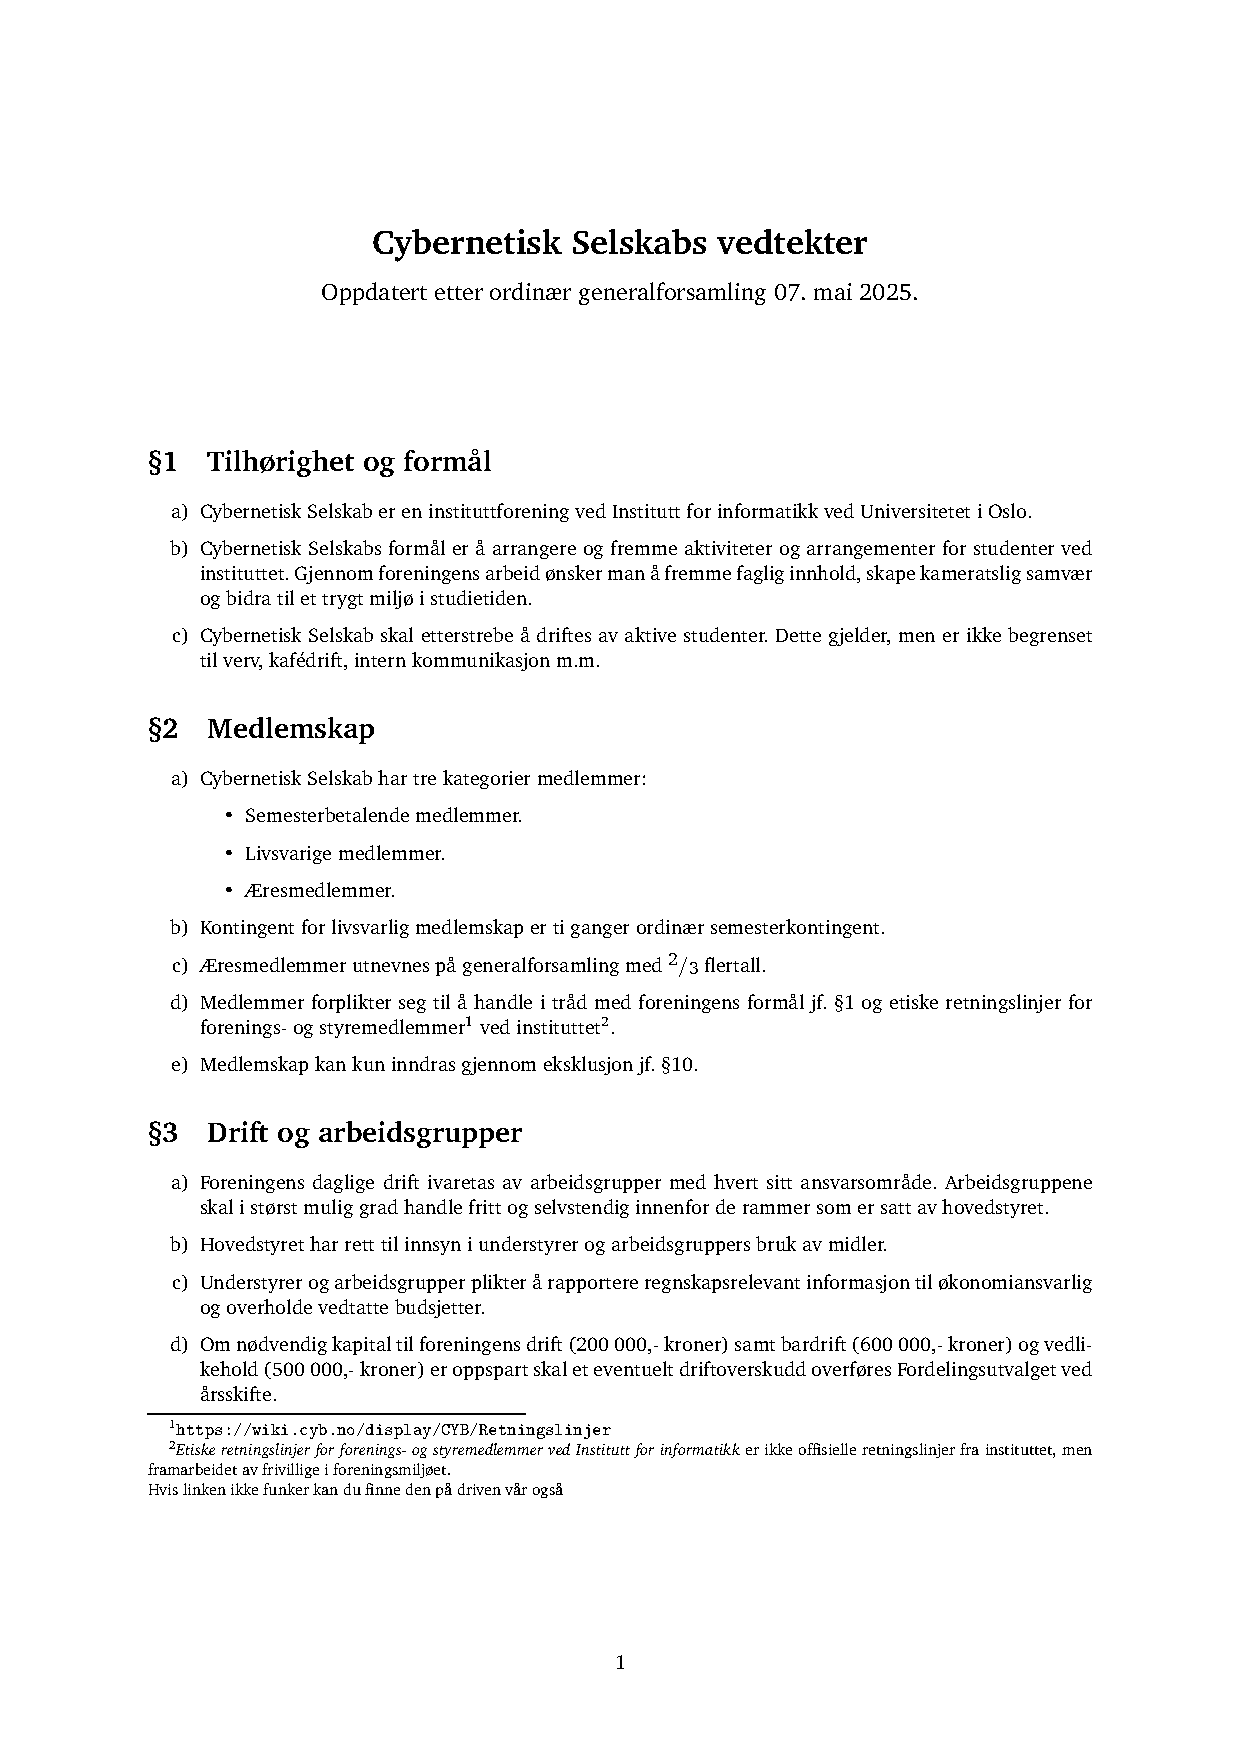
\includepdf[pages=-]{../vedtekter/vedtekter.pdf}

% TODO Fjern når ikke relevant
\phantomsection{}
\addcontentsline{toc}{section}{Vedtekter for Ifi-foreninger}
\includepdf[pages=-]{ifi_forening_vedtekter_2017.pdf}

\end{document}
